A continuación se detallará la estructura completa del punto de entrada de datos.  Éste componente del sistema también es conocido como \textit{Receiver} por ser su principal función el recibimiento y posterior almacenado de datos que provienen de fuentes externas al sistema.


\subsubsection{Diagrama de componentes}
La figura \ref{fig:diagrama_componentes_receiver} muestra el diagrama de todos los componentes que conforman el punto de entrada de datos.

El punto de entrada de datos está construido como una aplicación web que escucha peticiones del exterior y las procesa para almacenar los datos que recibe en diferentes puntos de almacenamiento.
\begin{landscape}
	\begin{figure}[ht]
		\centering
		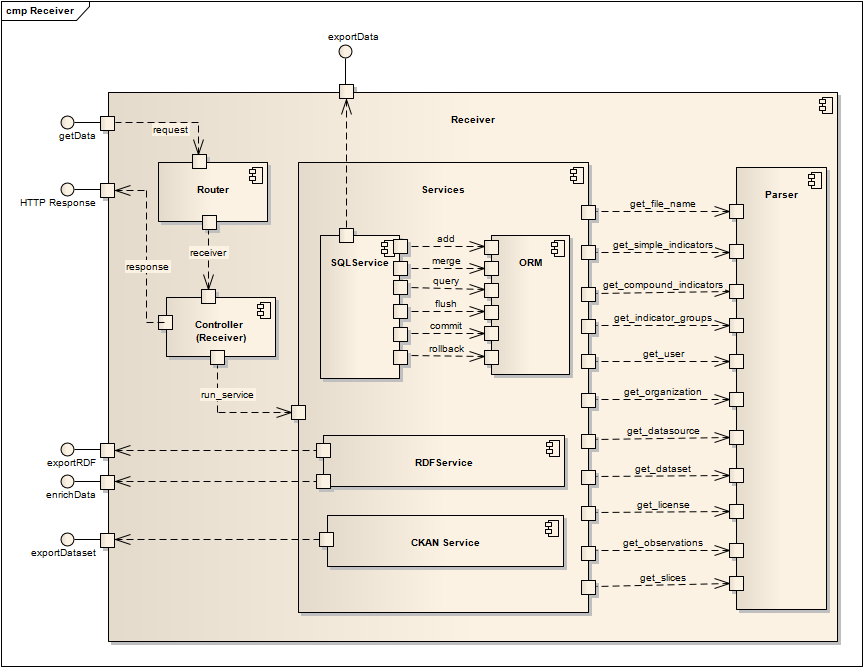
\includegraphics[height=\textwidth]{arquitectura/receiver_view}
		\caption{Diagrama de componentes del punto de entrada de datos}
		\label{fig:diagrama_componentes_receiver}
	\end{figure}
\end{landscape}


\subsubsection{Descripción de los componentes}
Tras haber mostrado el diagrama de los componentes que forman parte del punto de entrada de datos es el momento de explicar el papel que juega cada uno de ellos.

\begin{description}
	\item[Router]  El enrutador se encarga de dirigir las peticiones HTTP que provienen del exterior hacia el controlador.  También es el encargado de responder a las peticiones que no se correspondan con ningún controlador, o que no utilicen un verbo adecuado.
	\item[Controller (Receiver)]  El controlador se encarga de las peticiones de inserción de datos.  Su misión es comprobar si la petición que recibe tiene una forma adecuada y llamar a los distintos servicios para que procesen los datos.
	\item[Parser]  El parser es el encargado de transformar los datos provenientes de las peticiones externas a un modelo de datos que será utilizado por los servicios para realizar los diferentes procesados.  El modelo de datos será visto con más detalle en la sección ``\nameref{diseno_modelo_datos}'' de éste mismo capítulo.
	\item[SQLService]  El servicio de SQL se encarga de procesar los datos que llegan al punto de entrada y generar las consultas necesarias para almacenarlos en una base de datos relacional.  Éste servicio delega la generación de consultas SQL al ORM.
	\item[ORM]  El Mapeador Objeto-Relacional actúa como una capa de abstracción sobre la base de datos y permite al desarrollador trabajar con objetos sin necesidad de ocuparse de su transformación al modelo relacional.
	\item[RDFService]  El servicio de RDF se encarga de procesar los datos que llegan al punto de entrada y generar los grafos RDF que serán almacenados en el servidor semántico.
	\item[CKANService]  El servicio de CKAN se encarga de procesar los datos que llegan al punto de entrada y generar los metadatos que se almacenan en el catálogo de datos.
\end{description}


\subsubsection{Relacion entre los componentes}
Las peticiones provenientes de los importadores llegan al enrutador.  El enrutador redirige las peticiones que utilicen un verbo adecuado (POST) hacia el controlador, quien comprueba si la petición cuenta con todos los parámetros necesarios.

Si la petición cuenta con los parámetros adecuados, el controlador llama a cada uno de los servicios para que realicen su trabajo.  Los distintos servicios utilizarán a su vez el parser para convertir la información que proviene de la petición a un modelo de datos con el que ellos pueden trabajar.


\subsubsection{Interfaces y puertos}
A continuación se detallarán las interfaces y puertos de los componentes que forman parte del punto de entrada de datos. 

\paragraph{Receiver} \hfill \\
La tabla \ref{interfaces_receiver_receiver} muestra el detalle de las interfaces del \textit{Receiver}.
\begin{longtable}[c]{|p{25mm}|p{20mm}|p{30mm}|p{60mm}|}
 \caption{Vista del punto de entrada de datos - interfaces del \textit{Receiver}.\label{interfaces_receiver_receiver}}\\

 %Cabecera en la primera pagina
 \hline
 	Interfaz & Tipo & Tecnología & Propiedades\\
 \hline
 \hline
 \endfirsthead
 %Cabecera en el resto de páginas
 \hline
 \multicolumn{4}{|c|}{Continuación de la tabla \ref{interfaces_receiver_receiver}}\\
 \hline
 	Interfaz & Tipo & Tecnología & Propiedades\\
 \hline
 \hline
 \endhead
 %Tabla
 \hline
 \endfoot
 
	\textbf{HTTP Request} & Proveída & Servicio web REST & Recibe las peticiones procedentes del exterior \\
	\hline
		
	\textbf{HTTP Response} & Proveída & Servicio web REST & Responde a las peticiones HTTP recibidas \\
	\hline
	
	\textbf{exportRDF} & Requerida & API del servidor semántico & Exporta en formato RDF los datos recibidos de la petición \\
	\hline
	
	\textbf{exportData} & Requerida & Consultas a base de datos & Exporta en formato SQL los datos recibidos de la petición \\
	\hline
	
	\textbf{exportDataset} & Requerida & API del catálogo de datos & Exporta el catálogo de datos recibido de la petición junto con sus metadatos \\
	\hline
	
	\textbf{enrichData} & Requerida & Consultas SPARQL & Enriquece los datos mediante consultas SPARQL a servidores semánticos externos \\
\hline
\hline

 \end{longtable}
 
 
 \paragraph{Router} \hfill \\
 La tabla \ref{interfaces_receiver_router} muestra el detalle de las interfaces del \textit{Router}.
 \begin{longtable}[c]{|p{25mm}|p{20mm}|p{30mm}|p{60mm}|}
  \caption{Vista del punto de entrada de datos - interfaces del \textit{Router}.\label{interfaces_receiver_router}}\\
 
  %Cabecera en la primera pagina
  \hline
  	Interfaz & Tipo & Tecnología & Propiedades\\
  \hline
  \hline
  \endfirsthead
  %Cabecera en el resto de páginas
  \hline
  \multicolumn{4}{|c|}{Continuación de la tabla \ref{interfaces_receiver_router}}\\
  \hline
  	Interfaz & Tipo & Tecnología & Propiedades\\
  \hline
  \hline
  \endhead
  %Tabla
  \hline
  \endfoot
  
 	\textbf{HTTP Request} & Puerto de entrada & Servicio web REST & Recibe las peticiones procedentes del exterior \\
 	\hline
 	
 	\textbf{receiver} & Puerto de salida & Llamada a método & Pasa la petición al controlador correspondiente tras haber comprobado que utiliza el verbo adecuado \\
 \hline
 \hline
 
  \end{longtable}
  
\paragraph{Controller} \hfill \\
La tabla \ref{interfaces_receiver_controller} muestra el detalle de las interfaces del \textit{Controller}.

\begin{longtable}[c]{|p{25mm}|p{20mm}|p{30mm}|p{60mm}|}
 \caption{Vista del punto de entrada de datos - interfaces del textit{Controller}.\label{interfaces_receiver_controller}}\\
   %Cabecera en la primera pagina
 \hline
 	Interfaz & Tipo & Tecnología & Propiedades\\
 \hline
 \hline
 \endfirsthead
 %Cabecera en el resto de páginas
 \hline
 \multicolumn{4}{|c|}{Continuación de la tabla \ref{interfaces_receiver_controller}}\\
 \hline
 	Interfaz & Tipo & Tecnología & Propiedades\\
 \hline
 \hline
 \endhead
 %Tabla
 \hline
 \endfoot
 	
 	\textbf{receiver} & Puerto de entrada & Llamada a método & Recibe la petición procedente el enrutador y comprueba si incluye todos los parámetros necesarios \\
 	\hline
 	
 	\textbf{run service} & Puerto de salida & Llamada a método & Ejecuta la funcionalidad de un servicio \\
 	\hline
 	
 	\textbf{response} & Puerto de salida & Servicio web REST & Envía una respuesta con un código de error HTTP adecuado en función del éxito o no en el procesamiento de la petición. \\
\hline
\hline
 
\end{longtable}


\paragraph{Interfaces comunes a todos los servicios} \hfill \\
La tabla \ref{interfaces_receiver_services} muestra el detalle de las interfaces comunes a todos los servicios.

\begin{longtable}[c]{|p{25mm}|p{20mm}|p{30mm}|p{60mm}|}
 \caption{Vista del punto de entrada de datos - interfaces comunes a todos los servicios.\label{interfaces_receiver_services}}\\
 %Cabecera en la primera pagina
 \hline
 	Interfaz & Tipo & Tecnología & Propiedades\\
 \hline
 \hline
 \endfirsthead
 %Cabecera en el resto de páginas
 \hline
 \multicolumn{4}{|c|}{Continuación de la tabla \ref{interfaces_receiver_services}}\\
 \hline
 	Interfaz & Tipo & Tecnología & Propiedades\\
 \hline
 \hline
 \endhead
 %Tabla
 \hline
 \endfoot
 
 	\textbf{run service} & Puerto de entrada & Llamada a método & Comienza la ejecución del servicio \\
 	\hline
 	
 	\textbf{get file name} & Puerto de salida & Llamada a método & Obtiene el nombre del fichero que contiene los datos en bruto \\
 	\hline
 	
 	\textbf{get simple indicators} & Puerto de salida & Llamada a método & Obtiene una lista de los indicadores simples obtenidos del fichero de datos \\
 	\hline
 	
 	\textbf{get compound indicators} & Puerto de salida & Llamada a método & Obtiene una lista de los indicadores compuestos obtenidos del fichero de datos \\
 	\hline
 	
  	\textbf{get user} & Puerto de salida & Llamada a método & Obtiene los del usuario que realiza la petición de inserción de datos \\
  	\hline
  	
  	\textbf{get organization} & Puerto de salida & Llamada a método & Obtiene la información sobre la organización que proporciona el fichero de datos \\
  	\hline
  	
   	\textbf{get datasource} & Puerto de salida & Llamada a método & Obtiene la información sobre la fuente de datos de la que procede el fichero de datos \\
   	\hline
   	
   	\textbf{get dataset} & Puerto de salida & Llamada a método & Obtiene la información sobre el propio fichero de datos\\
   	\hline
   	
   	\textbf{get license} & Puerto de salida & Llamada a método & Obtiene la información sobre la licencia bajo la que se publica el fichero de datos \\
   	\hline
   	
   	\textbf{get observations} & Puerto de salida & Llamada a método & Obtiene la lista de observaciones procedentes del fichero de datos \\
   	\hline
   	
   	\textbf{get slices} & Puerto de salida & Llamada a método & Obtiene la lista con las \textit{slices}\footnote{Para más información sobre las \textit{slices} véase la sección ``\nameref{concept:rdf_data_cube}'' perteneciente al capítulo \ref{chapter03}} procedentes del fichero de datos. \\
   	\hline
\hline
\hline
 
\end{longtable}


\paragraph{Interfaces del \textit{Parser}} \hfill \\
La tabla \ref{interfaces_receiver_parser} muestra el detalle de las interfaces pertenecientes al \textit{Parser}.

\begin{longtable}[c]{|p{25mm}|p{20mm}|p{30mm}|p{60mm}|}
 \caption{Vista del punto de entrada de datos - interfaces pertenecientes al \textit{Parser}.\label{interfaces_receiver_parser}}\\
 %Cabecera en la primera pagina
 \hline
 	Interfaz & Tipo & Tecnología & Propiedades\\
 \hline
 \hline
 \endfirsthead
 %Cabecera en el resto de páginas
 \hline
 \multicolumn{4}{|c|}{Continuación de la tabla \ref{interfaces_receiver_parser}}\\
 \hline
 	Interfaz & Tipo & Tecnología & Propiedades\\
 \hline
 \hline
 \endhead
 %Tabla
 \hline
 \endfoot
 	
 	\textbf{get file name} & Puerto de entrada & Llamada a método & Devuelve el nombre del fichero que contiene los datos en bruto \\
 	\hline
 	
 	\textbf{get simple indicators} & Puerto de entrada & Llamada a método & Devuelve una lista de los indicadores simples obtenidos del fichero de datos \\
 	\hline
 	
 	\textbf{get compound indicators} & Puerto de entrada & Llamada a método & Devuelve una lista de los indicadores compuestos obtenidos del fichero de datos \\
 	\hline
 	
  	\textbf{get user} & Puerto de salida & Llamada a entrada & Devuelve los del usuario que realiza la petición de inserción de datos \\
  	\hline
  	
  	\textbf{get organization} & Puerto de entrada & Llamada a método & Devuelve la información sobre la organización que proporciona el fichero de datos \\
  	\hline
  	
   	\textbf{get datasource} & Puerto de entrada & Llamada a método & Devuelve la información sobre la fuente de datos de la que procede el fichero de datos \\
   	\hline
   	
   	\textbf{get dataset} & Puerto de entrada & Llamada a método & Devuelve la información sobre el propio fichero de datos\\
   	\hline
   	
   	\textbf{get license} & Puerto de entrada & Llamada a método & Devuelve la información sobre la licencia bajo la que se publica el fichero de datos \\
   	\hline
   	
   	\textbf{get observations} & Puerto de entrada & Llamada a método & Devuelve la lista de observaciones procedentes del fichero de datos \\
   	\hline
   	
   	\textbf{get slices} & Puerto de entrada & Llamada a método & Devuelve la lista con las \textit{slices} procedentes del fichero de datos. \\
   	\hline
\hline
\hline
 
\end{longtable}


\paragraph{SQLService} \hfill \\
La tabla \ref{interfaces_receiver_sqlservice} muestra el detalle de las interfaces del \textit{servicio de SQL} que no han sido incluidas anteriormente en la tabla \ref{interfaces_receiver_services}.  

\begin{longtable}[c]{|p{25mm}|p{20mm}|p{30mm}|p{60mm}|}
	\caption{Vista del punto de entrada de datos - interfaces del \textit{servicio de SQL}.\label{interfaces_receiver_sqlservice}}\\
	%Cabecera en la primera pagina
		\hline
			Interfaz & Tipo & Tecnología & Propiedades\\
		\hline
		\hline
	\endfirsthead
	%Cabecera en el resto de páginas
		\hline
		\multicolumn{4}{|c|}{Continuación de la tabla \ref{interfaces_receiver_sqlservice}}\\
		\hline
			Interfaz & Tipo & Tecnología & Propiedades\\
		\hline
		\hline
	\endhead
	%Tabla
	\hline
	\endfoot
		\textbf{exportData} & Requerida & Consultas a base de datos & Exporta en formato SQL los datos recibidos de la petición \\
		\hline
		\textbf{add} & Puerto de salida & Llamada a método & Almacena los datos de un objeto del modelo en la base de datos \\
		\hline
		\textbf{merge} & Puerto de salida & Llamada a método & Actualiza los datos de un objeto del modelo en la base de datos \\
		\hline
		\textbf{query} & Puerto de salida & Llamada a método & Realiza una consulta a la base de datos y devuelve los resultados\\
		\hline
		\textbf{flush} & Puerto de salida & Llamada a método & Vuelca los cambios realizados en memoria a la base de datos \\
		\hline
		\textbf{commit} & Puerto de salida & Llamada a método & Cierra una transacción con la base de datos \\
		\hline
		\textbf{rollback} & Puerto de salida & Llamada a método & Deshace los cambios de la transacción en curso\\
		\hline
	\hline
	\hline
\end{longtable}


\paragraph{ORM} \hfill \\
La tabla \ref{interfaces_receiver_orm} muestra el detalle de las interfaces del \textit{ORM}.  

\begin{longtable}[c]{|p{25mm}|p{20mm}|p{30mm}|p{60mm}|}
	\caption{Vista del punto de entrada de datos - interfaces del \textit{ORM}.\label{interfaces_receiver_orm}}\\
	%Cabecera en la primera pagina
		\hline
			Interfaz & Tipo & Tecnología & Propiedades\\
		\hline
		\hline
	\endfirsthead
	%Cabecera en el resto de páginas
		\hline
		\multicolumn{4}{|c|}{Continuación de la tabla \ref{interfaces_receiver_orm}}\\
		\hline
			Interfaz & Tipo & Tecnología & Propiedades\\
		\hline
		\hline
	\endhead
	%Tabla
	\hline
	\endfoot
		\textbf{add} & Puerto de entrada & Llamada a método & Almacena los datos de un objeto del modelo en la base de datos \\
		\hline
		\textbf{merge} & Puerto de entrada & Llamada a método & Actualiza los datos de un objeto del modelo en la base de datos \\
		\hline
		\textbf{query} & Puerto de entrada & Llamada a método & Realiza una consulta a la base de datos y devuelve los resultados\\
		\hline
		\textbf{flush} & Puerto de entrada & Llamada a método & Vuelca los cambios realizados en memoria a la base de datos \\
		\hline
		\textbf{commit} & Puerto de entrada & Llamada a método & Cierra una transacción con la base de datos \\
		\hline
		\textbf{rollback} & Puerto de entrada & Llamada a método & Deshace los cambios de la transacción en curso\\
		\hline
	\hline
	\hline
\end{longtable}


\paragraph{RDFService} \hfill \\
La tabla \ref{interfaces_receiver_rdfservice} muestra el detalle de las interfaces del \textit{servicio de RDF} que no han sido incluidas anteriormente en la tabla \ref{interfaces_receiver_services}.  

\begin{longtable}[c]{|p{25mm}|p{20mm}|p{30mm}|p{60mm}|}
	\caption{Vista del punto de entrada de datos - interfaces del \textit{servicio de RDF}.\label{interfaces_receiver_rdfservice}}\\
	%Cabecera en la primera pagina
		\hline
			Interfaz & Tipo & Tecnología & Propiedades\\
		\hline
		\hline
	\endfirsthead
	%Cabecera en el resto de páginas
		\hline
		\multicolumn{4}{|c|}{Continuación de la tabla \ref{interfaces_receiver_rdfservice}}\\
		\hline
			Interfaz & Tipo & Tecnología & Propiedades\\
		\hline
		\hline
	\endhead
	%Tabla
	\hline
	\endfoot
		\textbf{exportRDF} & Requerida & API del servidor semántico & Exporta en formato RDF los datos recibidos de la petición \\
		\hline
		\textbf{enrichData} & Requerida & Consultas SPARQL & Enriquece los datos mediante consultas SPARQL a servidores semánticos externos \\
	\hline
	\hline
\end{longtable}


\paragraph{CKANService} \hfill \\
La tabla \ref{interfaces_receiver_ckanservice} muestra el detalle de las interfaces del \textit{servicio de CKAN} que no han sido incluidas anteriormente en la tabla \ref{interfaces_receiver_services}.  

\begin{longtable}[c]{|p{25mm}|p{20mm}|p{30mm}|p{60mm}|}
	\caption{Vista del punto de entrada de datos - interfaces del \textit{servicio de CKAN}.\label{interfaces_receiver_ckanservice}}\\
	%Cabecera en la primera pagina
		\hline
			Interfaz & Tipo & Tecnología & Propiedades\\
		\hline
		\hline
	\endfirsthead
	%Cabecera en el resto de páginas
		\hline
		\multicolumn{4}{|c|}{Continuación de la tabla \ref{interfaces_receiver_ckanservice}}\\
		\hline
			Interfaz & Tipo & Tecnología & Propiedades\\
		\hline
		\hline
	\endhead
	%Tabla
	\hline
	\endfoot
		\textbf{exportDataset} & Requerida & API del catálogo de datos & Exporta el catálogo de datos recibido de la petición junto con sus metadatos \\
	\hline
	\hline
\end{longtable}